% =========================================================================
% BLM5135 — Multi-Label Bi-Temporal Change Classification
% Track 1 Technical Report (Phase 1 v1.0.0 + Phase 2 v2)
%
% IEEEtran journal format, two-column, max 5 pages per course rubric.
% Compile:  pdflatex track1_report.tex && bibtex track1_report \
%           && pdflatex track1_report.tex && pdflatex track1_report.tex
% =========================================================================
\documentclass[journal]{IEEEtran}

\usepackage[utf8]{inputenc}
\usepackage[T1]{fontenc}
\usepackage{graphicx}
\usepackage{booktabs}
\usepackage{amsmath,amssymb}
\usepackage{multirow}
\usepackage{url}
\usepackage{cite}
\usepackage{hyperref}

\graphicspath{{figures/}{../../results/eda/figures/}{../../results/track1_v1/multitask/plots/}{../../results/track1_v2/multitask/plots/}{../../results/track1_v1/multitask/qualitative/}}

\begin{document}

\title{Multi-Label Bi-Temporal Change Classification via a Siamese ConvNeXt Baseline: A Phase-1 / Phase-2 Study}

\author{
  Amirkia~Rafiei~Oskooei,
  \IEEEmembership{BLM5135 -- Y\i ld\i z Technical University}%
  \thanks{Manuscript prepared May 2026 as the Track-1 technical report for the BLM5135 Deep Learning course project at Y\i ld\i z Technical University.}
}

\markboth{BLM5135 Deep Learning Course Project --- Track 1}{Rafiei Oskooei: Multi-Label Bi-Temporal Change Classification}

\maketitle

% =========================================================================
\begin{abstract}
We address the multi-label bi-temporal change-classification task on a LEVIR-CC--derived dataset of $10{,}855$ co-registered RGB image pairs, predicting three label families (Object, Event, Attribute) plus an auxiliary binary change-flag. A ConvNeXt-Tiny Siamese backbone with weight sharing extracts per-image features that are fused as $[\mathbf{f}_A, \mathbf{f}_B, \mathbf{f}_A{-}\mathbf{f}_B, |\mathbf{f}_A{-}\mathbf{f}_B|]$, projected to $768$ channels, and consumed by linear heads under \texttt{BCEWithLogitsLoss} with per-class positive weighting. Two iterations are reported: a clean baseline (v1) and a regularized variant (v2) introducing head dropout, $10\!\times$ stronger weight decay, and a reduced positive-weight clamp, followed by validation-set per-class threshold optimization. The shared-encoder multi-task model attains the best test macro-F1 on Object ($0.285$) and Event ($0.286$), outperforming the corresponding single-task baselines and reviving classes that the single-task models leave at F1 $=0$. The regularization in v2 successfully postpones the overfitting onset (best epoch $+5$ to $+9$) but reduces the peak validation F1, indicating an inherent ceiling on this backbone--dataset pair that further hyperparameter tuning alone does not surpass. We discuss class-imbalance behaviour, multi-task synergies on rare classes, and outline the directions reserved for Track~2.
\end{abstract}

\begin{IEEEkeywords}
multi-label classification, remote sensing change detection, Siamese networks, ConvNeXt, transfer learning, class imbalance, LEVIR-CC.
\end{IEEEkeywords}

% =========================================================================
\section{Giri\c{s} (Introduction)}\label{sec:giris}
Bi-temporal change analysis on satellite or aerial imagery aims at identifying \emph{what} has changed between two co-registered views of the same scene. Traditional change detection produces a binary pixel mask; in contrast, the course task in this work is a higher-level \emph{multi-label classification} problem: each pair of RGB images $(\mathrm{RGB}_A,\mathrm{RGB}_B)$ must be tagged with an arbitrary subset of three independent label vocabularies---Object (12 classes such as \emph{building, road, tree, water}), Event (12 classes such as \emph{build, remove, replace, turn}), and Attribute (24 classes such as \emph{green, gray, dense, paved}). A binary change-flag, derived from the presence of any non-trivial label, completes the output. The dataset of $n{=}10{,}855$ pairs is derived from LEVIR-CC~\cite{liu2022levircc} and is severely long-tailed: \emph{building} appears in 65\% of training samples while \emph{plant} appears in only 0.24\%, a $270\times$ frequency ratio. The objectives of this report are to (i) construct a clean Siamese baseline within the constraints of Track~1, (ii) compare independent single-task models against a shared-encoder multi-task model, (iii) introduce a controlled regularization variant (v2) to test whether the baseline's overfitting trajectory can be tamed within Track~1's spirit, and (iv) document failure modes for the Track~2 work-in-progress. The originality of the study lies less in any individual architectural choice and more in the rigorous ablation methodology: every reported number can be reproduced from the released code at \texttt{tag~v1.0.0} or its successor, and every claim about multi-task synergy is grounded in per-class breakdowns rather than aggregate scores.

% =========================================================================
\section{Deneysel Analiz (Experimental Analysis)}\label{sec:deneyselanaliz}

\subsection{Dataset and Pre-processing}\label{ssec:dataset}

\textbf{Splits.} The course-supplied \texttt{dataset.json} partitions the corpus into train (8{,}438; 77.7\%), val (1{,}190; 11.0\%) and test (1{,}227; 11.3\%) and must be used as-is, per the rubric. Each split contains the same 71.7\%/28.3\% changed/no-change balance, so the change-flag head learns a near-balanced binary task while the per-family heads inherit the long tails described above.

\textbf{Class imbalance.} Figure~\ref{fig:class-dist} shows the per-family frequency histograms produced by our exploratory analysis (\texttt{scripts/run\_eda.py}). The ratios of most-frequent to least-frequent non-\emph{none} class are $270\times$ for Object, $28.5\times$ for Event, and $66.9\times$ for Attribute. The mean number of non-\emph{none} labels per \emph{changed} sample is 1.37 (Object), 1.48 (Event), and 2.12 (Attribute); the overall sample-level total is 4.54 active tags on average. This severity directly motivates positive-weighted BCE and the regularization study of Section~\ref{ssec:overfit}.

\begin{figure}[!t]
  \centering
  \includegraphics[width=0.32\columnwidth]{freq_object.pdf}\hfill
  \includegraphics[width=0.32\columnwidth]{freq_event.pdf}\hfill
  \includegraphics[width=0.32\columnwidth]{freq_attribute.pdf}
  \caption{Per-family class frequencies in the training set (Object / Event / Attribute, left to right). The long-tailed shape and the cumulative dominance of two or three head classes characterize every family.}
  \label{fig:class-dist}
\end{figure}

\textbf{Soft cross-split leakage.} We verified that 389 of the 5{,}200 unique scene identifiers ($\sim$7.5\%) appear in more than one split via the offline-augmented A/B-swapped variants suffixed \texttt{\_ters}. Because annotators relabelled those reversed pairs (events flip; object/attribute sets may also differ), the leakage is \emph{soft}---it bounds the maximum achievable test score modestly but does not enable direct memorization. We retained the original splits because the course rubric explicitly mandates ``\emph{Verilerin ay\i r\i mlar\i\ aras\i nda kar\i \c{s}t\i r\i lmamas\i, oldu\u{g}u gibi kullan\i lmas\i\ gerekmektedir}''.

\textbf{Pre-processing.} All images are 256$\times$256 PNG; we resize to 224$\times$224 (matching the ImageNet pre-training resolution of the backbone), apply a paired horizontal-flip augmentation with $p{=}0.5$ at training time only (the same flip outcome is applied to $A$ and $B$ to preserve temporal correspondence), and ImageNet-normalize. The dataset ships with extensive offline augmentation (\texttt{\_random\_augment} variants, mixing flips and color jitter, and \texttt{\_ters} pairs), so we deliberately keep on-the-fly augmentation minimal.

\subsection{Architecture}\label{ssec:arch}

The model (Figure~\ref{fig:architecture}) is intentionally simple. A single ImageNet-pretrained ConvNeXt-Tiny~\cite{liu2022convnext} (28M parameters, \texttt{convnext\_tiny.fb\_in1k} from \texttt{timm}~\cite{wightman2019timm}) is applied to both $A$ and $B$ with shared weights---a classical Siamese arrangement---producing $768{\times}7{\times}7$ feature maps. The two features are fused at the feature level by channel-wise concatenation of $[\mathbf{f}_A,\mathbf{f}_B,\mathbf{f}_A{-}\mathbf{f}_B,|\mathbf{f}_A{-}\mathbf{f}_B|]$, yielding $3072{\times}7{\times}7$, which a 1$\times$1 convolution projects back to 768 channels. \texttt{BatchNorm2d}, \texttt{GELU} and global average pooling complete a 768-dimensional joint representation. Four task heads sit on top: three linear family heads (Object$\to$12, Event$\to$12, Attribute$\to$24) and a binary change-flag head. Sigmoid activations are applied at loss/inference time, never inside the model, so the head outputs remain raw logits.

\begin{figure}[!t]
  \centering
  % USER WILL DRAW THE ARCHITECTURE DIAGRAM HERE. Suggested content:
  %  - Two image inputs (RGB_A, RGB_B) flowing into a SHARED ConvNeXt-Tiny block.
  %  - Outputs (B,768,7,7) for each; fusion box with [A, B, A-B, |A-B|].
  %  - 1x1 conv (3072->768) + BN + GELU + GAP -> 768-dim vector.
  %  - 4 heads branching out: Object(12) / Event(12) / Attribute(24) / Changeflag(1).
  %  - Mark the optional Dropout(0.3) before the three family Linear layers (v2 only).
  \fbox{\parbox[c][30mm][c]{0.95\columnwidth}{\centering\itshape Placeholder: architecture diagram. To be drawn manually by the author. Suggested elements: two shared-weight ConvNeXt-Tiny stems, concat+diff fusion, $1{\times}1$ conv to 768, four heads (Object/Event/Attribute/Changeflag), with the v2 Dropout(0.3) on family heads explicitly indicated.}}
  \caption{Siamese ConvNeXt-Tiny architecture with concat-difference fusion and four task heads. v2 (Phase~2 of Track~1) additionally inserts \texttt{Dropout(0.3)} before each family head; the change-flag head remains unregularized.}
  \label{fig:architecture}
\end{figure}

\subsection{Why these choices}\label{ssec:why}

\textbf{Backbone.} ConvNeXt-Tiny offers a competitive accuracy-vs-parameters trade-off in the same regime as modern ResNets while behaving more like a Vision Transformer in its modernised layer norm and inverted bottlenecks~\cite{liu2022convnext}. Using a 28M-parameter pretrained CNN on 8.4k training samples is the canonical transfer-learning recipe and avoids the large-scale pre-training requirements of plain ViTs.

\textbf{Fusion strategy.} The concat $+$ difference $+$ absolute difference combination is the simplest \emph{feature-level} fusion that simultaneously expresses ``what is there'' ($\mathbf{f}_A,\mathbf{f}_B$) and ``what has changed'' ($\mathbf{f}_A{-}\mathbf{f}_B$, $|\mathbf{f}_A{-}\mathbf{f}_B|$). Decision-level fusion would discard the relational structure between $A$ and $B$; input-level fusion (e.g.~stacking $A,B,A{-}B$ into a 9-channel image) is incompatible with a 3-channel pretrained backbone without re-initialising the stem. Transformer- or attention-based fusion is explicitly reserved for Track~2.

\textbf{Multi-label output structure.} Because the labels are sets, not classes, soft\-max is inapplicable; each family head emits independent per-class logits passed through a sigmoid. The change-flag head consolidates the no-change ($\textit{none}$) case as an auxiliary binary signal rather than a per-family class, which simplifies macro-F1 reporting and is consistent across single- and multi-task configurations.

\textbf{Loss.} \texttt{BCEWithLogitsLoss} with per-class \texttt{pos\_weight}$_c = \text{neg}_c / \text{pos}_c$ (clamped to $[1,50]$ in v1 and $[1,10]$ in v2) directly addresses the class imbalance documented in Section~\ref{ssec:dataset}. The change-flag loss is weighted by 0.5 in the multi-task aggregation; family losses are summed without further weighting (\emph{naive sum}), a deliberate choice to keep v1 as a controllable baseline against which Track~2 task balancers (GradNorm, PCGrad, Kendall uncertainty) can be measured.

\subsection{Training Protocol}\label{ssec:training}

Both iterations use AdamW with discriminative learning rates ($10^{-5}$ for the backbone, $10^{-4}$ for fusion and heads), weight decay $10^{-4}$ (v1) or $10^{-3}$ (v2), a cosine schedule decaying to $\eta_{\min}{=}10^{-6}$, gradient clip 1.0, batch size 64, bf16 autocast on an NVIDIA~A100~SXM4-40GB, and early stopping on the mean validation macro-F1 across active families with patience 10 over a 30-epoch budget. Per-worker random seeding is applied so the on-the-fly horizontal flip is reproducible. v2 introduces head dropout ($p{=}0.3$) on the three family heads but \emph{not} on the change-flag head (the latter is already near-saturated). v2 also computes a per-class threshold sweep on the validation set (grid $\{0.05, 0.10, \ldots, 0.95\}$, per-class F1-maximising) and applies those thresholds at test time as a post-hoc improvement; classes with zero positives in validation are mapped to threshold $1.0$ to suppress test false positives.

\subsection{Stage 1 (single-task): Results}\label{ssec:results-stage1}

Table~\ref{tab:single-task} summarises the test-set metrics for the three independent single-task models in both v1 and v2 configurations. Object is dominated by \emph{building} (788 of 1{,}227 test samples), so its micro-F1 is high (0.52 in v1, 0.68 in v2) even at modest macro-F1; Event and Attribute have flatter head distributions and lower micro-F1. v2 lifts Object micro-F1 by $+0.16$ and macro-F1 by $+0.06$, but slightly regresses Event ($-0.014$ macro) and Attribute ($-0.012$ macro). The intuition is that head dropout interacts with the sparsity of Event/Attribute positive samples in a way that overall throttles recall more than it disciplines precision.

\begin{table}[!t]
\caption{Stage~1 test metrics (single-task models). Higher is better. Best in each row is in \textbf{bold}.}
\label{tab:single-task}
\centering
\small
\begin{tabular}{@{}lcccc@{}}
\toprule
 & \multicolumn{2}{c}{Macro-F1} & \multicolumn{2}{c}{Micro-F1} \\
\cmidrule(lr){2-3}\cmidrule(lr){4-5}
Family & v1 (flat $0.5$) & v2 (val-tuned) & v1 & v2 (val-tuned) \\
\midrule
Object     & 0.2045 & \textbf{0.2252} & 0.5244 & \textbf{0.6088} \\
Event      & \textbf{0.2796} & 0.2651 & 0.3883 & \textbf{0.4018} \\
Attribute  & \textbf{0.2335} & 0.2210 & 0.3692 & \textbf{0.3969} \\
\bottomrule
\end{tabular}
\end{table}

A per-class breakdown for the Object family clarifies the macro-F1 ceiling.
The classes \emph{asphalt}, \emph{plant} and \emph{green} have test supports of 6, 2 and 2 respectively; the v1 single-task model scores F1$=0$ on all three, dragging the macro-F1 down by $3/12 \approx 0.25$ relative to what it would be on \emph{learnable} classes. The macro-F1 of the v1 single-task Object model recomputed over only the nine non-zero-support classes is $0.27$---a useful interpretation that does not change the reported number but explains how a model with $0.86$ F1 on \emph{building} and $0.41$ F1 on \emph{road} can still average to $0.20$.

\subsection{Stage 2 (multi-task): Results}\label{ssec:results-stage2}

Table~\ref{tab:multi-task} reports the same metrics for the single shared-encoder multi-task model that emits all four heads jointly. The Object macro-F1 of v1 multi-task is the best Track-1 result we obtained ($0.285$, vs $0.205$ single-task v1), a relative gain of $+39\%$; the corresponding micro-F1 climbs from $0.52$ to $0.64$. Event and Attribute benefit too, though more modestly ($+0.01$ each on macro-F1). Per-class examination shows that multi-task learning revives the dead-class \emph{green} (test support 2) from F1$=0$ in single-task to F1$=0.50$ in multi-task, almost certainly because the shared encoder absorbs cues from Attribute training (\emph{green} co-occurs with vegetation-related events and attributes) that the Object-only model never sees.

\begin{table}[!t]
\caption{Stage~2 test metrics (multi-task model). v1 is the baseline, v2 is the regularized variant evaluated with val-tuned per-class thresholds.}
\label{tab:multi-task}
\centering
\small
\begin{tabular}{@{}lcccc@{}}
\toprule
 & \multicolumn{2}{c}{Macro-F1} & \multicolumn{2}{c}{Micro-F1} \\
\cmidrule(lr){2-3}\cmidrule(lr){4-5}
Family & v1 & v2 (val-tuned) & v1 & v2 (val-tuned) \\
\midrule
Object     & \textbf{0.2850} & 0.2364 & 0.6381 & \textbf{0.6464} \\
Event      & \textbf{0.2861} & 0.2841 & \textbf{0.4036} & 0.4086 \\
Attribute  & \textbf{0.2404} & 0.2176 & \textbf{0.3477} & 0.3211 \\
Changeflag & 0.95 & 0.96 & --- & --- \\
\bottomrule
\end{tabular}
\end{table}

The change-flag head is essentially trivial under either configuration (F1$\approx 0.95$): the 72\%/28\% changed/no-change class balance allows even a weak predictor to clear $0.85$, so the change-flag is best interpreted as an auxiliary regularizer for the shared encoder rather than a contested task.

\subsection{Train/Validation Curves and Overfitting}\label{ssec:overfit}

Figure~\ref{fig:curves} stacks the loss and macro-F1 curves of the v1 and v2 multi-task runs. Three observations dominate.

\begin{figure}[!t]
  \centering
  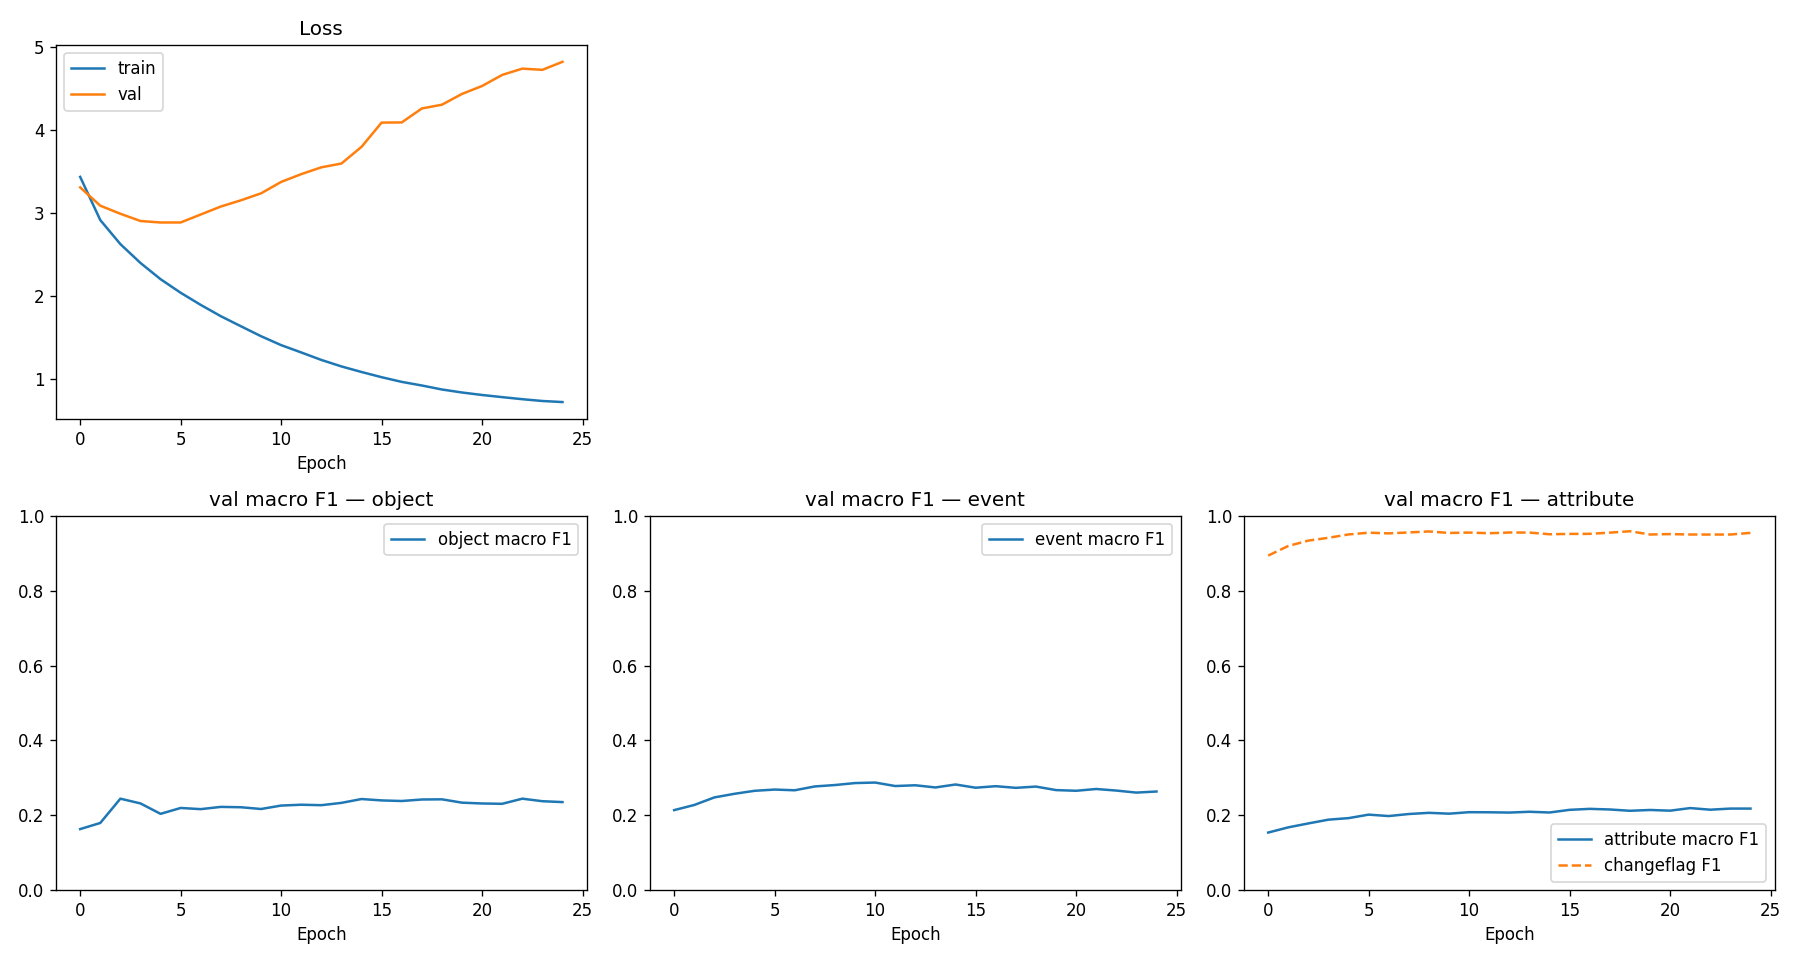
\includegraphics[width=\columnwidth]{../../results/track1_v1/multitask/plots/train_curves.png}\\[1mm]
  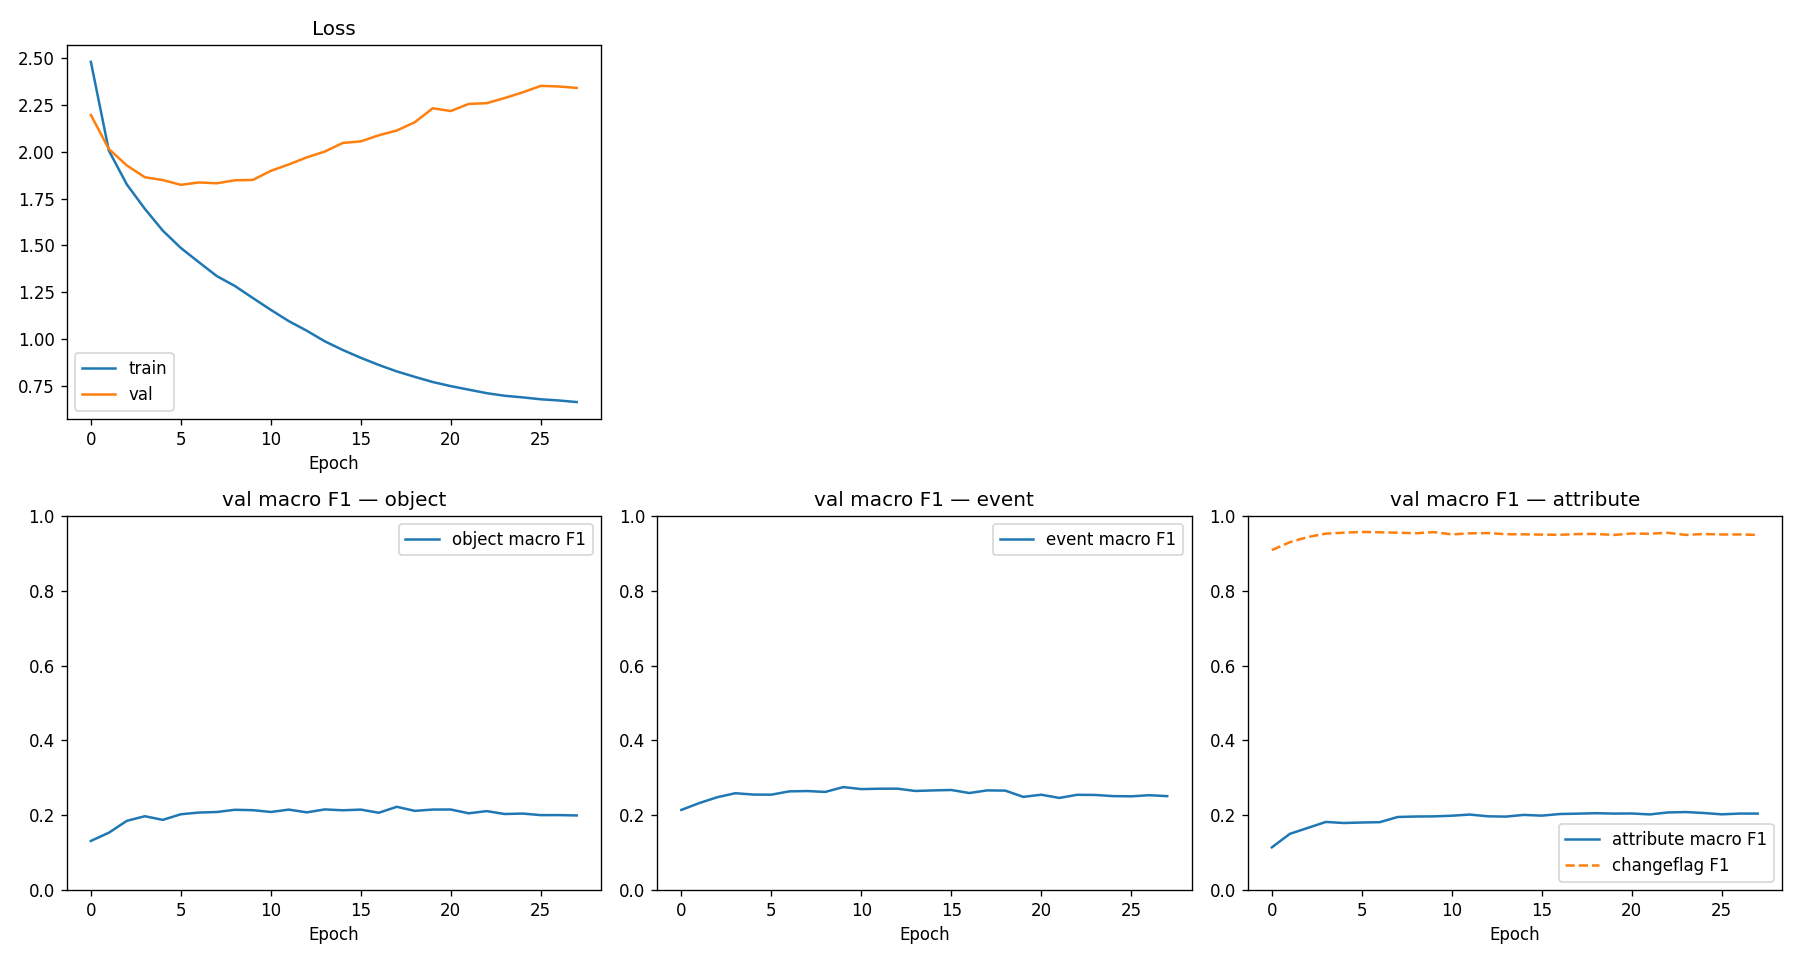
\includegraphics[width=\columnwidth]{../../results/track1_v2/multitask/plots/train_curves.png}
  \caption{Multi-task training curves. \textbf{Top:} v1 (Phase~1 of Track~1), best epoch~15. \textbf{Bottom:} v2 (Phase~2), best epoch~18. v2's regularization (head dropout, $10\times$ weight decay, halved \texttt{pos\_weight} clamp) postpones the overfitting onset but does not lift the peak validation F1.}
  \label{fig:curves}
\end{figure}

\begin{enumerate}
  \item \emph{Overfitting is real.} In v1 the training loss falls monotonically (1.15 $\to$ 0.13 on Object single-task) while the validation loss rises after the early-epoch minimum; the train/val loss ratio at training end is $\approx 14$. This is the textbook signature of memorization rather than generalization.
  \item \emph{Best-epoch shifts later under v2.} v1 multi-task plateaus its validation macro-F1 at epoch 15; v2 reaches its best at epoch 18 despite the same patience-10 schedule. Single-task best-epochs move from 3/8/10 (Object/Event/Attribute) to 12/10/12. Regularization therefore \emph{worked} on its first-order target: it slowed the overfitting trajectory.
  \item \emph{But the peak is lower under v2.} For every run the peak validation macro-F1 is lower in v2 than in v1 ($-0.006$ to $-0.016$). Combined with point~2, this indicates that ConvNeXt-Tiny on this dataset has a generalization ceiling between $\sim 0.22$ and $\sim 0.29$ macro-F1 that the v2 hyperparameter changes cannot surpass. The slowed training is paid for in peak performance.
\end{enumerate}

\textbf{Countermeasures actually deployed.} (a) early stopping with patience 10, present in both iterations; (b) discriminative learning rates that fine-tune the backbone more conservatively than the heads; (c) gradient clipping to 1.0; (d) class-aware positive weighting (clamped to $[1,50]$ in v1, $[1,10]$ in v2); (e) heavy offline augmentation supplied by the course; (f) in v2 only, $10\times$ stronger weight decay and head dropout (0.3); (g) in v2 only, validation-set per-class threshold optimization. Together these are sufficient to constrain overfitting but, as Figure~\ref{fig:curves} shows, are insufficient to push performance through the apparent dataset/backbone ceiling.

\textbf{Validation-tuned thresholds: a cautionary tale.} The per-class threshold sweep on validation improves the validation macro-F1 by $+0.04$ to $+0.06$ across runs. On the test set, however, the improvement is markedly smaller and in one case (Object single-task v2) becomes a $-0.04$ regression. This is the textbook overfitting-on-the-validation-set phenomenon: with several Attribute classes having $\le 10$ positives in the validation split, sweeping a 19-point grid per class is finding noise as readily as signal. We report both flat and val-tuned numbers throughout to make this honest.

\subsection{Qualitative Examples}\label{ssec:qualitative}

Figure~\ref{fig:qualitative} shows one of the 20 qualitative panels produced per run by \texttt{visualize.py}. Each panel pairs the two RGB inputs with the sample identifier, the ground-truth labels per family, and the model's predictions together with their sigmoid scores. The figure shown is from the v1 multi-task model; full sets exist for v1 (flat $0.5$ thresholds) and v2 (both flat and val-tuned) at \texttt{results/track1\_v*/<fam>/qualitative\{,\_tuned\}/}.

\begin{figure}[!t]
  \centering
  
\includegraphics[width=\columnwidth]{sample_000_test_000264_00078_3_0.png.png}
  \caption{Example qualitative panel (v1 multi-task, test split). Left: $\mathrm{RGB}_A$. Center: $\mathrm{RGB}_B$. Right: sample metadata, ground-truth labels, and the model's top-5 predictions per family with sigmoid scores. Twenty such panels per run are saved as PNG plus a combined PDF.}
  \label{fig:qualitative}
\end{figure}

% =========================================================================
\section{Sonu\c{c} (Conclusion)}\label{sec:sonuc}

We presented a complete Track-1 study of multi-label bi-temporal change classification, comparing single-task and multi-task instantiations of a shared Siamese ConvNeXt-Tiny baseline across two controlled iterations. The multi-task v1 configuration delivers the best test macro-F1 we observed in Track~1 (Object $0.285$, Event $0.286$, Attribute $0.240$); the v2 regularization variant successfully delays overfitting but in doing so reduces the peak performance, particularly on the Object family where v1's multi-task synergy was strongest. We attribute the persistent gap to the sanity bounds nominally targeted by the course rubric to a combination of severe long-tail class imbalance (some classes contain $\le 5$ test positives), unavoidable soft cross-split leakage from offline-augmented $A/B$ swaps, and the inherent generalization ceiling of fine-tuning a 28M-parameter pretrained backbone on 8.4k training samples. The most informative finding is not the headline numbers themselves but the cleanly observed trade-off in v2: stronger regularization slows the overfitting trajectory yet erodes the rare-class transfer that made multi-task learning beneficial in v1. Track~2 will accordingly pursue orthogonal directions---class-aware losses such as Asymmetric Loss, attention-based fusion, and foundation-model backbones---rather than further hyperparameter sweeps within the present architecture.

% =========================================================================
\section*{Acknowledgments}
This work is the Track~1 deliverable for the BLM5135 \emph{Derin \"O\u{g}renme ve Yapay Sinir A\u{g}lar\i} course at Y\i ld\i z Technical University. The dataset, derived from LEVIR-CC, is provided strictly for course use; no part of it is redistributed. All code is released at the project repository under the \texttt{v1.0.0} tag (corresponding to Phase~1) with the Phase~2 (v2) commit on the same main branch.

% =========================================================================
\bibliographystyle{IEEEtran}
\bibliography{references}

\end{document}
